%% CSAI 2026 submission draft (bylined, dual-column).
%% Target: 5--5.5 pages within the 4--6 page dual-column limit.
%% Source of truth: affective-sedimentation-csai-2026-sprint-final.zh.md
%% Numeric claims must match reports/paper_number_lock.json.
%% Figures: fig_E_items; fig_N_seeds; fig_E_grid; fig_N_dirseed.

\documentclass[sigconf]{acmart}

%% Rights management information.
\setcopyright{none}
\acmYear{2026}
\acmDOI{}

%% Proceedings information.
\acmConference[CSAI 2026]{10th International Conference on Computer Science and Artificial Intelligence}{December 18--21, 2026}{Beijing, China}
\acmISBN{}

\usepackage{booktabs}
\usepackage{graphicx}
\usepackage{microtype}
\usepackage{amsmath}
%% [H] pins each single-column float to the paragraph break where it is declared, so no
%% float drifts above its owning heading, past its discussion, or into another float.
\usepackage{float}

%% acmart v2.19 dropped the uppercase run on sigconf \section headings; the shipped
%% sample-sigconf.pdf still shows them. Restore it, leaving \subsection in title case.
\makeatletter
\def\@secfont{\bfseries\Large\section@raggedright\MakeUppercase}
\makeatother

%% The default 10pt above and below each display environment is more air than
%% this measure needs.
\setlength{\abovedisplayskip}{4pt plus 2pt minus 2pt}
\setlength{\belowdisplayskip}{4pt plus 2pt minus 2pt}
\setlength{\abovedisplayshortskip}{2pt plus 1pt}
\setlength{\belowdisplayshortskip}{2pt plus 1pt}

%% Absorbs the handful of sub-7pt overfull lines this two-column measure produces around
%% hyphenated compounds and bracketed citations, without rewording anything to fit.
\emergencystretch=1em

\setlength{\textfloatsep}{6pt plus 2pt minus 4pt}
\setlength{\floatsep}{6pt plus 2pt minus 4pt}
\setlength{\intextsep}{6pt plus 2pt minus 4pt}
\setlength{\dbltextfloatsep}{6pt plus 2pt minus 4pt}
\setlength{\dblfloatsep}{6pt plus 2pt minus 4pt}
\renewcommand{\dblfloatpagefraction}{0.7}
\renewcommand{\floatpagefraction}{0.7}
\renewcommand{\topfraction}{0.85}
\renewcommand{\dbltopfraction}{0.85}
\renewcommand{\bottomfraction}{0.5}
\renewcommand{\textfraction}{0.1}
\setcounter{topnumber}{3}
\setcounter{dbltopnumber}{2}
\setcounter{totalnumber}{5}

%% acmart leaves a full inter-item skip between reference entries. The entries are already
%% hanging-indented, so the skip is redundant as a separator and only costs page.
\setlength{\bibsep}{0pt plus 0.2ex}

\begin{document}

\title{Affective Sedimentation: A Controlled Proof-of-Mechanism for History-Driven Behavioral Modulation in an LLM Agent}

\author{Zexian Xiong}
\affiliation{%
  \institution{University of Nottingham Ningbo China}
  \city{Ningbo}
  \state{Zhejiang}
  \country{China}
}
\email{shyzx4@nottingham.edu.cn}

\author{Yan Li}
\authornote{\ Corresponding author. Email: sylvie.li@nottingham.edu.cn}
\affiliation{%
  \institution{University of Nottingham Ningbo China}
  \city{Ningbo}
  \state{Zhejiang}
  \country{China}
}
\email{sylvie.li@nottingham.edu.cn}

\renewcommand{\shortauthors}{Xiong and Li}

\begin{abstract}
Long-horizon LLM agents normally carry the past as retrieved text, so anything that persists has to be replayed in the context window. This study is to explore a narrower question: can a slow affect state, updated outside the model and shown to it only as background metadata, shift forced choices while prompts, probes and option semantics stay fixed? The mechanism we build is \emph{affective sedimentation}. A three-layer recurrence updates slow P/A/D coordinates outside the model, and a fixed renderer writes them into the prompt as background text that names no action. Two pre-registered experiments test that text interface, not the recurrence behind it. Experiment~E contrasts affect-labeled endpoint metadata with numerically matched sensor metadata and no history (180 observations). Experiment~N is the only one that involves history; it contrasts history-derived rendered state against a same-memory origin render $R_1[(0,0,0)]$ under fixed scripted \texttt{EVENT\_MEMORY} (576 observations). Both gate suites passed on one Qwen snapshot with author-defined probes ($\theta_E{=}0.2678$, $p_E{=}0.0156$; $\theta_N{=}0.1042$, $p_N{=}0.00391$; MES${=}0.10$), with each $p$-value at its theoretical lower bound. The effect is real but narrow. Nine of the fifteen probes never varied across the injected endpoints, returning the maximum order-corrected choice score in every cell. Of the remaining effect, $89.2\%$ lies below the origin render, and one history direction, low activation, carries $73.3\%$ of the history-state estimand. The unlabeled control channel did not respond to its own coordinates at all. We report the saturation of the instrument alongside the effect it limits, and make no claim about internal emotion, personality, or cross-model generality.
\end{abstract}

\begin{CCSXML}
<ccs2012>
 <concept>
  <concept_id>10010147.10010257</concept_id>
  <concept_desc>Computing methodologies~Machine learning</concept_desc>
  <concept_significance>500</concept_significance>
 </concept>
 <concept>
  <concept_id>10010147.10010178</concept_id>
  <concept_desc>Computing methodologies~Artificial intelligence</concept_desc>
  <concept_significance>500</concept_significance>
 </concept>
</ccs2012>
\end{CCSXML}

\ccsdesc[500]{Computing methodologies~Machine learning}
\ccsdesc[500]{Computing methodologies~Artificial intelligence}

\keywords{large language models, LLM agents, affective state, prompt interface, controlled pilot}

\maketitle

\section{Introduction}

Longer-horizon interactions pose a concrete design question: can an agent carry a slow, history-updated tendency across turns, or is it limited to retrieving episodic logs? The mechanisms usually used to carry anything forward act through the context window: in-context exemplars~\cite{brown2020language}, intermediate reasoning~\cite{wei2022chain}, retrieved event records~\cite{park2023generative}. All of them reinstate past content. None maintains a separate variable that is recomputed from an engineered appraisal map and re-injected without explicit recall. We call that process \emph{affective sedimentation}.

Adding transcript memory cannot settle whether such a state channel differs from episodic recall; that requires controlled evidence at the interface where the state is injected. We test one interface-level question: whether \emph{externally rendered affect-state metadata}, slow P/A/D coordinates updated recurrently and inserted as background text, can modulate forced-choice tendencies when prompts, probes and option semantics remain fixed. We contribute a renderer exposing those coordinates as background metadata that names no action; a numerically matched control block relabelling the same coordinates as meaningless sensor channels; a same-memory zero-state ablation injecting $R_1[(0,0,0)]$ alongside an identical \texttt{EVENT\_MEMORY} string $M(H)$; and pre-registered gates read in the fixed order $D\rightarrow E\rightarrow N$.

Both gate suites passed. Affect-labeled metadata shifted choices where numerically matched sensor metadata did not, and history-derived state shifted them further than a same-memory origin render, each at the smallest $p$-value its design could produce. How far it extends is a separate question. Most of our probe set saturated at the choice-score ceiling, itself a methodological finding: an instrument can pass its own pre-registered gates and still be informative on only a minority of its items. All readouts are order-corrected choice scores (CS) on probes we wrote ourselves and one model snapshot, so we do not treat the P/A/D axes as a validated scale and do not generalise to other models.

\subsection{Related Work}
While prior simulations pursue long-horizon behavior via memory retrieval~\cite{park2023generative} and recent agents via consolidated long-term memory~\cite{zhong2024memorybank}, standard LLM steering relies on in-context conditioning~\cite{brown2020language}. This control surface is highly sensitive: meaning-preserving formatting changes can shift task accuracy by up to 76 points~\cite{sclar2024quantifying}. Our placebo is built against that sensitivity, holding the rendered numbers fixed and varying only the labels attached to them. Prior work injecting affect appends emotional \emph{instructions} and measures task accuracy~\cite{li2023emotional}, elicits an emotion and scores the decisions that follow~\cite{mozikov2024eai,ho2026induced}, or studies the mechanism through which emotion shapes agent behaviour~\cite{sun2026emotion}. We inject state that names no action and measure forced-choice tendency. Our manipulation sits at the prompt interface, not the representation level. It needs no access to weights or hidden states and therefore applies to a commercial snapshot, at the cost of leaving label salience confounded with affect semantics. Affect here is an engineered external controller variable with pre-specified dynamics, not an inferred latent property, described in the role-play register recommended for dialogue agents~\cite{shanahan2023roleplay,shanahan2024talking}. A close recent work is Sentipolis~\cite{fu2026sentipolis}, which builds emotion-aware agents for social simulation; our object is the interface, not the architecture.

\section{Method}

The method comprises a controller producing slow coordinates, a text renderer, and a pre-registered analysis plan. In Experiment~N (576 observations) a fixed 200-event history $H$ passes through gate~D into the deterministic controller $\epsilon\rightarrow m\rightarrow s$; Experiment~E (180) skips that stage and sets the coordinates directly. Either way the coordinates are rendered as background text $R_1[z(s)]$, paired with a probe in AB and BA orders, and read back as a JSON choice scored into CS; the gates then apply in the fixed order $D\rightarrow E\rightarrow N$.

The stage from $H$ to $s(H)$ is engineered, not tested: gate~D only checks that the implementation reproduces its specification, so no behavioral result below can confirm or refute it. The model never sees $s$, only the rendered text $R_1[z(s)]$, with $z(\cdot)$ a fixed three-decimal signed rendering. Behavioral evidence therefore enters at exactly one place.

\subsection{Three-Layer Controller and Endpoints}
For event index $t{=}0,\ldots,199$, each appraisal vector $a_t$ updates:
\begin{align}
\epsilon_{t+1}&=\lambda\epsilon_t+(1-\lambda)a_t,\\
m_{t+1}&=(1-\alpha)m_t+\alpha\epsilon_{t+1},\\
s_{t+1}&=(1-\gamma_t)s_t+\gamma_t m_{t+1},
\end{align}
with $\gamma_t=\gamma_0/(1+t/\tau)^p$ and $\epsilon_0{=}m_0{=}s_0{=}(0,0,0)$. Parameters are $\lambda{=}0.40$, $\alpha{=}0.10$, $\gamma_0{=}0.02$, $\tau{=}50$, $p{=}1$, $T{=}200$. Feedback gain $\beta$ is zero and state is unclipped. Golden checks reproduce the protocol's specified timings, with $\kappa_{200}$ matching to $<10^{-12}$ absolute error.

Both experiments place their levels in that coordinate space, though only N reaches them by running the recurrence. Pure-axis endpoints P$\pm$, A$\pm$, D$\pm$, and a shared origin map to $z\in[-1,+1]$ via asymmetric bounds and three-decimal half-to-even rounding (signed ASCII; $-0.000\rightarrow{+}0.000$). Experiment~E injects endpoints directly and reports slopes in CS per rendered-$z$ span; Experiment~N injects $z(s_{200}(H))$ or the origin at $t{=}200$, with both cells sharing identical $M(H)$.

\subsection{Appraisal Map, Histories, and Rendering}
A fixed action table maps peer actions to OCC-style listener labels~\cite{ortony1988cognitive} and P/A/D increments. Non-neutral triples mirror the OCC-to-PAD mapping by Gebhard and Kipp~\cite{gebhard2006plausible} over Mehrabian's axes~\cite{mehrabian1996pad}, with a layered temporal decomposition~\cite{gebhard2005alma}. Because this source interpolates absent values by similarity, our mapping is an \emph{engineered appraisal mapping}, not a validated psychometric scale.

Each 200-action history deterministically generates both \texttt{EVENT\_\allowbreak MEMORY} and the appraisal stream. Formal Experiment~N uses eight hash-derived seeds (14, 24, 5, 18, 22, 13, 1, 26). These seeds permute the within-block ordering of one fixed event multiset, so cumulative action counts are identical across seeds and rendered $z$ differs only marginally. Seed-level claims therefore evaluate \emph{memory realization}, not compositional diversity. The affect renderer $R_1$ exposes coordinates as \texttt{LONG\_TERM\_\allowbreak AFFECT}; the active placebo uses unlabeled \texttt{ROOM\_\allowbreak METADATA} with identical numbers and parallel wording, including the same instruction to treat the block as background, but declaring its channels meaningless where the affect block supplies a decoding key. The formal snapshot is \texttt{qwen3.7-\allowbreak flash-\allowbreak 2026-07-15}.

\subsection{Prompts, Probes, and Estimands}
Each payload concatenates: role sentence; optional \texttt{EVENT\_\allowbreak MEMORY} (N only); metadata; scenario; counterbalanced options (AB/BA); and a strict JSON instruction. Models exhibit systematic preferences over option identifiers~\cite{zheng2024robust,zhao2021calibrate}; AB/BA averaging cancels the first-order component, and the discordance gates bound what survives. Experiment~E uses fifteen formal items (five per axis). Experiment~N replays nine hash-selected IDs ($9\subset15$), a same-domain state ablation.

For a complete AB/BA pair, $y{=}1$ if the semantic high option is chosen; $\mathrm{CS}=(y_{\mathrm{AB}}+y_{\mathrm{BA}})/2\in\{0,0.5,1\}$. $\mathrm{CS}_{b}(c)$ denotes CS under block $b$ at endpoint $c$. For axis $d$, probe $j$, and span $\Delta z_d$:
\begin{equation}
e_{d,j} = \frac{\mathrm{CS}_{\mathrm{affect}}(d{+})-\mathrm{CS}_{\mathrm{affect}}(d{-})}{\Delta z_d} - \frac{\mathrm{CS}_{\mathrm{placebo}}(d{+})-\mathrm{CS}_{\mathrm{placebo}}(d{-})}{\Delta z_d}.
\end{equation}
The origin cells enter no estimand and are kept for diagnostics; $\theta_E=\mathrm{mean}_{d,j}\,e_{d,j}$ over the fifteen items.

In Experiment~N, across six directions $h$, the full-minus-zero contrast is:
\begin{equation}
n_{h,k,j} = \mathrm{sign}(h)\,\bigl(\mathrm{CS}_{\mathrm{full}}(h,k,j)-\mathrm{CS}_{\mathrm{zero}}(h,k,j)\bigr).
\end{equation}
Seed units are $N_k=\mathrm{mean}_{h,j}\,n_{h,k,j}$, and $\theta_N=\mathrm{mean}_k\,N_k$. We call a positive $N_k$ \emph{direction-signed consistency}: under the retained state, choices fall on the side the engineered history direction points to.

\subsection{Analysis Plan and Pre-registration}
Primary inference relies on one-sided exact sign-flip tests~\cite{ernst2004permutation} over the E item effects and N seed means, whose null is that each analysis unit is sign-symmetric about zero. The alternative is directional and was fixed before collection, so the tests cannot register a departure in the opposite direction. Each test enumerates all $2^m$ sign patterns over those units ($m{=}15$ for E, $m{=}8$ for N). These tests address departure from zero, not from MES${=}0.10$, a separate engineering threshold fixed before any formal result and applied to the point estimate alone. The items and seeds are fixed sets we defined, not samples, so both $p$-values are randomization summaries over that grid. Secondary axis-wise tests use Holm adjustment ($\alpha{=}0.05$)~\cite{holm1979simple}; 5{,}000-resample bootstrap intervals~\cite{efron1979bootstrap} describe finite-grid sensitivity.

Two constraints follow. First, each of the 756 formal observations was drawn once at temperature~$0$, which does not guarantee deterministic repeats~\cite{ouyang2025nondeterminism}. Within-condition variance therefore remains unestimated, and our uncertainty bounds reflect variation between analysis units. Stability gates verified repeat-stability of the \emph{extracted choice} on twelve development payloads repeated three times each; that claim does not extend to the 756 formal rows. Second, a unit at exactly zero is unchanged by flipping its sign, so attainable resolution is set by the number of moving units $k$, not $m$: the minimum $p$-value is $2^{-k}$, which certifies that those units share a sign and says nothing about magnitude.

We also fixed the interpretive order at $D\rightarrow E\rightarrow N$, sealed a manifest over the 756-observation schedule, and logged 836 completed rows: 756 formal plus 80 development or stability rows that enter no inference.

\section{Experiments}

The two experiments are not replications. Because E sets its endpoints by hand, it can show that the rendered interface moves choices without showing that any history would put the controller there. N derives its state from an event history instead, supplying the step E leaves untested.

\begin{table}[H]
  \caption{The two experimental schedules.}
  \label{tab:design}
  \centering
  \small
  \setlength{\tabcolsep}{3.2pt}
  \begin{tabular}{@{}lcc@{}}
    \toprule
    Factor & Experiment E & Experiment N \\
    \midrule
    Scientific contrast & affect vs placebo & full vs zero-state \\
    State source & pure-axis endpoints & $s_{200}(H)$ / origin \\
    Event memory $M(H)$ & absent & identical across cells \\
    Axes / directions & P, A, D (matched) & P$\pm$, A$\pm$, D$\pm$ \\
    Probes & 15 formal (5/axis) & 9 replay ($9\subset15$) \\
    Seeds & --- & 8 fixed IDs \\
    Analysis units & 15 item $e_{d,j}$ & 8 seed $N_k$ \\
    \bottomrule
  \end{tabular}
\end{table}

Table~\ref{tab:design} lists the two schedules side by side, from the manipulated contrast to each estimand's unit. Experiment~E withholds \texttt{EVENT\_MEMORY} and drives pure-axis endpoints, testing direction response within each probe family; it claims neither orthogonality nor discriminant validity. Experiment~N holds $M(H)$ identical across its two cells and varies only the rendered state, asking whether history-derived state adds tendency once memory is controlled. Its levels are the realized $s_{200}(H)$, not a fixed dose, so $\theta_N$ is not on $\theta_E$'s scale and the two must not be compared numerically. The axis rows differ for a related reason: E drives both endpoints and reads one slope per probe, while an engineered history points one way, so each axis splits into two signed directions. N's nine replay probes come from E's fifteen, so we can later read E's ceiling against N's blank directions.

They also differ in what they average over: E's unit is a probe, N's a history ordering. E therefore asks whether the effect holds across the probes we wrote, N across orderings of one event multiset; neither asks whether it holds across models, prompts or event sets.

Both schedules ran under one collection procedure: a single pre-planned interleaved batch, precluding result-gating; JSON formatting with tools and search disabled and no re-prompting for invalid outputs; and no selective exclusion of data. Every number below comes from that one pass over the schedule.

\section{Results}

Results come from two provenances, kept separate throughout: sealed rebuilds of the pre-registered gates and estimands, and read-only diagnostic recomputations over the same ledger, which enter no gate. We report the gates first, since they establish that anything moved at all, then the response profiles, which determine how broadly that movement can be read.

\subsection{Primary Gates and Estimands}

\begin{table}[H]
  \caption{Primary gates and estimands.}
  \label{tab:primary}
  \centering
  \small
  \setlength{\tabcolsep}{3.2pt}
  \begin{tabular}{@{}lcc@{}}
    \toprule
    Quantity / gate & E & N \\
    \midrule
    $\theta$ (mean effect) & 0.2678 & 0.1042 \\
    Exact sign-flip $p$ (one-sided) & 0.0156 & 0.00391 \\
    MES (${=}0.10$) pass & yes & yes \\
    Sign-flip pass ($p\leq0.05$) & yes & yes \\
    Pair completeness & 90/90 & 288/288 \\
    Invalid JSON (final) & 0 & 0 \\
    Position discordance (overall) & 0.122 & 0.167 \\
    Discordance pass (overall/axis) & yes & yes \\
    Units complete & 15/15 & 8/8 \\
    Bootstrap 95\% CI & per axis only & $[0.0208,\,0.212]$ \\
    \bottomrule
  \end{tabular}
\end{table}

Table~\ref{tab:primary} reports each experiment's estimand, its exact sign-flip $p$, and one row per pre-registered criterion; position discordance passes only if the overall rate is ${\leq}0.25$ and every axis ${\leq}0.35$. Every criterion is met in both columns, and blind integrity QC verified 756 formal rows, zero duplicate observation keys, zero invalid JSON, and raw SHA-256 prefix \texttt{13c9588a\ldots}. Neither estimand indicates how broadly the effect extends.

Both $p$-values sit exactly at the floors derived above: $2^{-6}$ over E's six non-zero effects, $2^{-8}$ over N's eight non-zero means. They certify sign concordance and nothing more, leaving the magnitude claim entirely to $\theta$ against MES. The floor also limits what this design could ever have shown: had only four items moved, the smallest attainable $p_E$ would have been $2^{-4}{=}0.0625$, above the $0.05$ level however large those four effects were. The E gate cleared it partly because six of the fifteen items moved at all, which the design never guaranteed.

\begin{figure}[H]
  \centering
  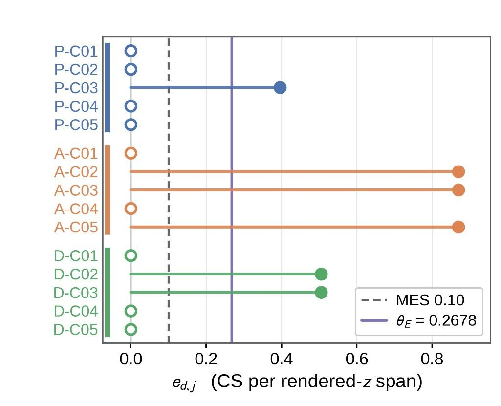
\includegraphics[width=0.92\columnwidth]{figures/fig_E_items.pdf}
  \Description{Horizontal lollipop chart of fifteen Experiment E contrasts grouped by axis. Nine markers sit exactly at zero. The six non-zero markers cluster on the activation axis.}
  \caption{The fifteen Experiment~E item units.}
  \label{fig:eitems}
\end{figure}

Figure~\ref{fig:eitems} plots the first average item by item: one row per probe, bar length the item's contrast $e_{d,j}$ in CS per rendered-$z$ span, open circles for exact zeros, a dashed MES line and a solid line at $\theta_E$. The distribution is sharply bimodal: nine items read exactly $0$, and the remaining six take only three positive values ($0.3965$, $0.5056$, $0.8696$), none negative. So $\theta_E{=}0.2678$ averages nine zeros with six values running from just under four to nearly nine times MES, describing no item in the set. The three largest fall on the activation axis, the first sign that the probe families do not behave alike. Those values are as much a property of the instrument as of the channel. CS is confined to $\{0,0.5,1\}$, so against a flat placebo an item can only return zero or a half or whole step of either sign, divided by its axis span. The six movers are whole steps on A ($1/1.150$) and half steps on D ($0.5/0.989$) and P ($0.5/1.261$): one value per axis, no within-axis variation. Agreement within an axis therefore reflects the lattice the measurement permits, not independent estimates converging on a shared slope. The mean over those six is $0.6694$, but that subset is defined by the outcome, so it is not a second estimand.

Since $\theta_E$ turned out to describe no item in its set, the second estimand needs the same reading before it can be trusted. Its unit is a history seed, not a probe, so the first reading does not carry over, and $\theta_N$ rests on eight numbers where $\theta_E$ rested on fifteen.

\begin{figure}[H]
  \centering
  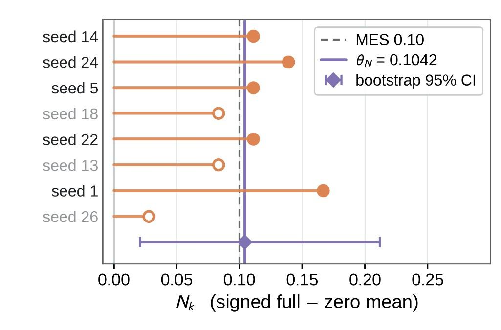
\includegraphics[width=0.92\columnwidth]{figures/fig_N_seeds.pdf}
  \Description{Horizontal lollipop chart of the eight Experiment N seed means in the pre-registered order. Three markers fall below MES.}
  \caption{The eight Experiment~N seed units.}
  \label{fig:nseeds}
\end{figure}

Figure~\ref{fig:nseeds} shows the second average seed by seed: one row per history seed in the pre-registered order, bar length the seed mean $N_k$, open circles for seeds below MES, and a diamond and bar for the bootstrap 95\% CI. The weakness here is of a different kind. All eight seeds are positive, which is why $p_N$ sits at its floor, but they are far from uniform, running from $0.0278$ to $0.1667$, a six-fold spread; three fall below MES (seeds $18$ and $13$ at $0.0833$, seed $26$ at $0.0278$) while the mean clears it by only $0.0042$. The N gate cleared on seed-equal aggregation, not on agreement among seeds that the effect is large; the interval $[0.0208,\,0.212]$ dips below MES for the same reason. A missing-data check over alternative pair rules did not change this: the fragility is in the spread across seeds.

Because the eight seeds are orderings of one event multiset, that spread is a range over orderings and not over histories in general. With one draw per observation the design cannot separate it from variation within a cell, so it bounds how stable the effect is without explaining what moves it.

Both figures leave the same question open. Nine E items at exactly $0$ and three N seeds below MES are consistent with an affect channel that reaches only part of the probe set, and with an instrument that cannot record what the channel does. The response levels answer this where the contrasts cannot: an item pinned at its maximum cannot register an increase, whereas one sitting mid-scale and holding still had room and did not use it. The next section therefore looks at the responses themselves.

\subsection{Response Profile of the Analysis Units}
\label{sec:profile}

\begin{figure}[H]
  \centering
  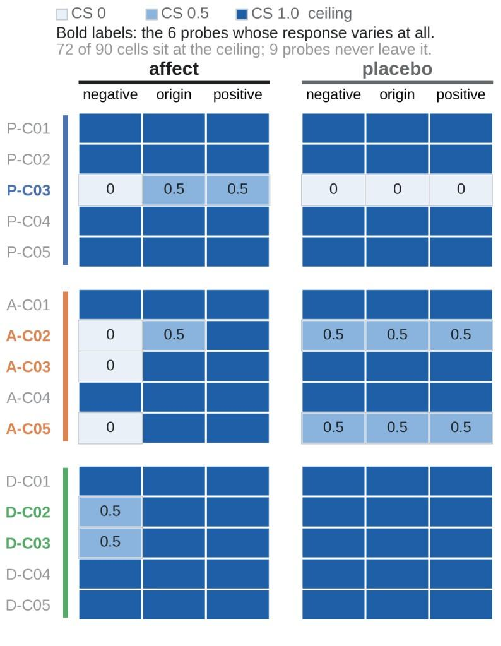
\includegraphics[width=0.92\columnwidth]{figures/fig_E_grid.pdf}
  \Description{Grid of ninety cells with fifteen probe rows in three axis blocks. Two panels side by side carry the affect block and the placebo block, each with three columns for the negative endpoint, the shared origin and the positive endpoint. The vast majority of cells are at choice score 1.0, and within the placebo panel every row is constant across its three columns.}
  \caption{The complete Experiment~E response surface, all ninety cells.}
  \label{fig:egrid}
\end{figure}

Figure~\ref{fig:egrid} gives the ninety response cells directly. Its fifteen rows are the probes in three axis blocks; its two panels are the affect and placebo blocks, each with three columns for the negative endpoint, the shared origin and the positive endpoint, at the same rendered coordinates in both: P $-0.545/0/+0.716$, A $-0.620/0/+0.530$ and D $-0.521/0/+0.468$. Shade encodes the order-corrected choice score, which takes only $0$, $0.5$ and $1.0$; cells below $1.0$ carry their value, so an unprinted cell is at $\mathrm{CS}{=}1.0$, and bold labels mark the six probes whose response varies.

Three things hold in that surface at once. First, 72 of the 90 cells sit at the ceiling and nine probes are at $1.0$ in all six of their cells. A ceiling-capped cell can only record a downward shift, so those nine rows carry no information about an upward effect, though they could have registered a downward one and did not. That answers the question above in one direction: the nine zeros of Figure~\ref{fig:eitems} are consistent with ceiling truncation and are not measurements of an absent effect. Second, saturation is uneven across axes (P 4/5, A 2/5, D 3/5) and runs opposite to the effect sizes, the most saturated axis carrying the smallest $\theta_E$ and the least saturated the largest. Headroom and effect size are therefore confounded, and axis heterogeneity cannot be attributed to the affect channel alone. Third, every row of the placebo panel is constant across its three columns, so the numerically matched but unlabeled channel produced no coordinate-dependent response and every $e_{d,j}$ comes from the affect block. This is an observation, not an estimate: $e_{d,j}$ subtracts the placebo slope away. E has no metadata-free condition, so the finding is that the placebo channel did not respond to its own numbers, not that inserting it had no effect.

If the effect is confined to a minority of probes, the next question is which part of the state range those probes respond to. Splitting each item's $e_{d,j}$ at the origin render, the negative-to-origin span contributes $0.2388$ against $0.0290$ from above, placing $89.2\%$ of the effect below the origin; the local half-slopes agree at $0.4579$ against $0.0629$, a ratio of $7.28$, though measured within each half-interval they are neither additive nor comparable to MES. Read alone, that says the affect channel drives choices away from the semantic-high option under negative coordinates. The headroom blocks that reading. Only two items could rise at the origin and only one, A-C02, did; the other thirteen were already at $\mathrm{CS}{=}1.0$ before the positive endpoint was rendered. The $89.2\%$ therefore measures the instrument as much as the channel.

\subsection{Axis-wise and Direction-wise Summaries}
\label{sec:axis}

\begin{figure}[H]
  \centering
  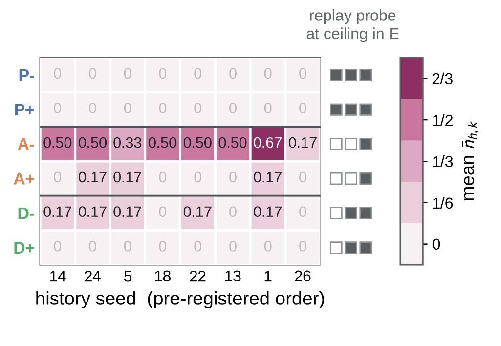
\includegraphics[width=0.92\columnwidth,trim=0 17 0 0,clip]{figures/fig_N_dirseed.pdf}
  \vspace{-8pt}
  \Description{Heatmap with six history-direction rows and eight history-seed columns, and a column of three ceiling markers per row at the right. The A-minus row is filled at every seed; D-minus at five and A-plus at three; the two valence rows and D-plus are zero throughout, and both valence rows carry three filled ceiling markers.}
  \caption{Experiment~N by history direction and seed.}
  \label{fig:ndirseed}
\end{figure}

We can read Experiment~N the same way. Figure~\ref{fig:ndirseed} arranges its 48 cells as six history-direction rows by eight seed columns in the pre-registered order; each cell is $\bar{n}_{h,k}$, the direction-signed full-minus-zero-state contrast averaged over the three replay probes on that direction's axis, printed in the cell and repeated as shade, so it takes only multiples of $1/6$. Beside each row sit those same three probes as squares, filled where the probe was already at the ceiling in E. Values are non-negative and 32 of the 48 cells are exactly $0$, so $\theta_N$ is concentrated in the way $\theta_E$ was: A$-$ supplies $73.3\%$ under seed-equal aggregation, D$-$ a further $16.7\%$ and A$+$ the remaining $10.0\%$, while P$+$, P$-$ and D$+$ contribute nothing.

The two empty valence rows look like an inert valence channel, but the marker column rules that reading out. Both rows carry three filled squares, so all three valence replay probes (P-C01, P-C02 and P-C05) were at the ceiling before Experiment~N began, and neither reading had room to move up. The rows are blank, not negative, so no downward departure appeared either. The same explanation covers D$+$ only partly, at two filled squares of three. The replay set was fixed by hash before any outcome was observed, so this is a property of the instrument. The figure therefore supports a strongly heterogeneous $\theta_N$ whose mass sits almost entirely on activation-related directions, and leaves the valence blank uninterpretable.

\begin{table}[H]
  \caption{Axis-wise secondary summaries.}
  \label{tab:axis}
  \centering
  \small
  \setlength{\tabcolsep}{2.8pt}
  \begin{tabular}{@{}lcccccc@{}}
    \toprule
    Axis & $\theta_E$ & E boot.\ 95\% & $\theta_N$ & Disc.\ E & Disc.\ N \\
    \midrule
    P & 0.079 & $[0.000,\,0.238]$ & 0.000 & 0.067 & 0.000 \\
    A & 0.522 & $[0.174,\,0.870]$ & 0.260 & 0.233 & 0.219 \\
    D & 0.202 & $[0.000,\,0.404]$ & 0.052 & 0.067 & 0.281 \\
    Overall & 0.2678 & --- & 0.1042 & 0.122 & 0.167 \\
    \bottomrule
  \end{tabular}
\end{table}

Table~\ref{tab:axis} reports both experiments per axis, with bootstrap intervals for Experiment~E only. All three E axes posted positive means, with activation dominating, and no axis rejected under Holm adjustment. That non-rejection was fixed by the design, not by the data: five items per axis put the best achievable $p$-value at $0.03125$, against a smallest Holm threshold of $0.0167$. The axis means are therefore descriptive only. N axis means are highly heterogeneous, blocking any claim of generalized three-axis consistency. A pre-registered dose-normalized sensitivity check leaves the direction intact at $0.1759$ CS per rendered-$z$, positive for all eight seeds; measured per rendered-$z$ instead of direction-corrected CS, it is not comparable to MES and enters no gate.

\section{Discussion}

Every pre-registered gate passed, and within those limits the result reads as a proof of mechanism: affect-labeled metadata produced steeper slopes than numerically matched sensor metadata, and replacing history-derived state with the origin render, while holding event memory fixed, reduced direction-signed consistency. That ablation is possible because event-memory text and slow-state metadata are decoupled. Neither experiment departed against the injected direction, and most non-moving items were already at ceiling. Yet the gates test completeness, thresholds, sign consistency and position bias, not construct validity; the effect was asymmetric, concentrated in activation-targeted probes and, in E, confined to six unsaturated items.

Two ambiguities qualify that reading. First, E compares an affect block with a decoding key against a placebo that declares identical coordinates meaningless. Despite the placebo's flat response, affect semantics remain confounded with label salience, a live concern given LLMs' formatting sensitivity~\cite{sclar2024quantifying} and token bias~\cite{zhao2021calibrate}. N has an analogous ambiguity: with identical 200-event memory, only the full cell is internally coherent, so the contrast may reflect memory--state agreement rather than the sedimented state.

Second, activation had both the largest effect and the highest discordance ($0.233$). A probe pegged at $\mathrm{CS}{=}1.0$ is mechanically concordant, making low discordance and ceiling saturation related measures. Activation items also oppose acting now to waiting, wording close to what the label \texttt{A} already carries. The data therefore show that the activation-targeted probe family moved, not that an activation channel did.

Saturation leaves unresolved whether the ceiling belongs to the fifteen items or to forced-choice probing more generally. In one exploratory comparison, $6$ of $18$ development cells were at ceiling, against $72$ of $90$ formal Experiment~E cells. This shows that the same authoring process can yield headroom, not why the formal set saturated; three probes are not a sample. Those rows enter no estimand, gate or interval: flipping them leaves all formal cells, both estimand sets and both gate objects bit-identical. Remaining limits include unvalidated P/A/D operationalizations, a finite grid and a single provider snapshot. Background-only wording and stability checks address instruction leakage and provider drift~\cite{chen2024drift}, but not construct threats.

\subsection{Future Work}
The next study should pre-register a development probe pool screened for headroom at the origin render and replicate the locked contrasts on an additional model snapshot. A decoding-key-preserving label permutation would separate affect semantics from label salience; a magnitude-matched state that breaks the history--state mapping would distinguish the rendered-state contrast from memory--state agreement. These controls should precede any claim of cross-model generality.

\subsection{Ethics and Disclosure}
Probes use fictional scenarios with no human participants, and no personal or user data was collected at any stage. We evaluate a single commercial snapshot to test an interface design, not to endorse proprietary behavior.

\section{Conclusion}

Within a single-model, forced-choice pilot, affect-labeled metadata modulated choices beyond an active placebo, and history-derived state modulated them above a same-memory origin render. Both are contrasts on one probe grid, and inside it the footprint was asymmetric: concentrated in the activation-targeted probes and truncated by extensive instrument saturation. The next version needs a probe set with room to move, and the response surface reported here shows what that instrument would have to avoid.

\bibliographystyle{ACM-Reference-Format-unsrt}
\bibliography{refs}

\end{document}
